\documentclass[]{aiaa-tc}% insert '[draft]' option to show overfull boxes

 \usepackage{varioref}%  smart page, figure, table, and equation referencing
 \usepackage{wrapfig}%   wrap figures/tables in text (i.e., Di Vinci style)
 \usepackage{threeparttable}% tables with footnotes
 \usepackage{dcolumn}%   decimal-aligned tabular math columns
  \newcolumntype{d}{D{.}{.}{-1}}
 \usepackage{nomencl}%   nomenclature generation via makeindex
  \makeglossary

  \usepackage{graphicx}
  \usepackage{caption}
  \usepackage{subcaption}
  \usepackage[toc,page]{appendix}
  \usepackage{pdfpages}
%  \usepackage{listings}
  
% \usepackage{subfigure}% subcaptions for subfigures
% \usepackage{subfigmat}% matrices of similar subfigures, aka small mulitples
 \usepackage{fancyvrb}%  extended verbatim environments
  \fvset{fontsize=\footnotesize,xleftmargin=2em}
 \usepackage{lettrine}%  dropped capital letter at beginning of paragraph
 \usepackage[export]{adjustbox}
 \usepackage{url}

 \title{GPU acceleration of wall distance calculation for
   computational fluid dynamics codes}
 \author{
   Nathan A. Wukie\thanks{Graduate student researcher, School of Aerospace Systems, ML 70, 
     Cincinnati, OH, AIAA Student Member.},
   \ Vasanth Ganapathy\thanks{Student, University of Cincinnati},
   \ Chris Park\thanks{Student, University of Cincinnati} \\
   {\normalsize\itshape
     University of Cincinnati, Cincinnati, OH, 45221, USA}\\
 }

 % Data used by 'handcarry' option
 %\AIAApapernumber{YEAR-NUMBER}
 %\AIAAconference{Conference Name, Date, and Location}
 %\AIAAcopyright{\AIAAcopyrightD{YEAR}}

 % Define commands to assure consistent treatment throughout document
 \newcommand{\eqnref}[1]{(\ref{#1})}
 \newcommand{\class}[1]{\texttt{#1}}
 \newcommand{\package}[1]{\texttt{#1}}
 \newcommand{\file}[1]{\texttt{#1}}
 \newcommand{\BibTeX}{\textsc{Bib}\TeX}

% Add highlighting - Wukie
\usepackage{color,soul}

\begin{document}

\maketitle

%\begin{abstract}
%Insert abstract
%\end{abstract}

%\section*{Nomenclature}

%\begin{tabbing}
%  XXX \= \kill% this line sets tab stop
%  $\rho$ \> Density \\
%  $\delta(f)$ \> Dirac delta function \\
%  $H(f)$ \> Heaviside function\\
%  $T_{ij}$ \> Lighthill stress tensor \\
%  $P_{ij}$ \> Compressive stress tensor \\
%  $u$ \> X-velocity \\
%  $v$ \> Y-velocity \\
%  $p'$ \> Pressure fluctuation\\
%  $x$ \> Tensor coordinate\\
%  $t$  \> Time\\
%  $c_o$ \> Reference speed of sound\\[5pt]
%  \textit{Subscript}\\
%  $i,j$ \> Tensor indices \\
%  $n$ \> Normal component\\
% \end{tabbing}

\section{Introduction}
\lettrine[nindent=0pt]{C}{omputational} fluid dynamics(CFD) is a branch of
simulation sciences that focuses on predicting fluid flows based on a
set of governing physical equations. There are many different methods
for accomplishing this that span both, different sets of governing
equations, in addition to different numerical methods for computing a
solution. Some different sets of equations that can be solved include
the potential flow equation, streamfunction-vorticity equations, Euler
equations, and Navier-Stokes equations. Analytical solutions to these
sets of equations are often not available except in some extremely
simple cases. Interesting geometries require a discretized
approach. Some common discretization methods include Finite Difference,
Finite Volume, and Finite Element methods. 

This research effort is focused on a problem for a subset
of those methods. In particular, we are interested in efficient wall
distance calculation algorithms to support Reynolds-Averaged
Navier-Stokes(RANS) solvers using a cell-centered, Finite Volume discretization with a
moving mesh capability.

\subsection{Background}

\subsubsection{Reynolds-Averaged Navier-Stokes Equations}
The Reynolds-Averaged Navier-Stokes(RANS) equations govern viscous, laminar
and turbulent flows. For turbulent flows, the turbulence is accounted
for via a turbulence model, which usually takes the
form of an additional partial differential equation or sometimes a set
of partial differential equations that solve for turbulent working
variables.

One general method for formulating these turbulence models is to
include ``production'' and ``destruction'' terms for the turbulent
working variables. In this way, phenomena that typically increase
turbulence, such as vorticity, will ``produce'' a turbulence effect by
increasing the turbulent working variable. One variable that governs such
turbulence production/destruction terms is the distance of a grid cell to
the nearest solid wall; simply known as the wall distance, $d_{wall}$.\cite{allmaras:12}


\subsubsection{Cell-centered, Finite Volume discretization}
The numerical method that this investigation directly supports is a
cell-centered, finite volume discretization, although it could be
readily extended to other methods with some modifications. The finite
volume method relies on an integral form of the governing equations,
and the method we are interested in stores all variables at the center
of each computational cell. The values in each cell can then be
updated, based on boundary fluxes computed at the interface of each
computational cell.\cite{hirsch:94} The value of interest here is the $d_{wall}$
variable required by the turbulence model.

\subsubsection{Moving mesh calculation}
Some investigations that use fluid simulations are interested in moving
body problems such as store separation for aircraft, and rotating
machinery, among others. One way to accomplish this is to use
body-local grids that overlap a background grid as shown in Figure~\ref{f:chimera_grid}.\cite{galbraith:13phd} In this way, the body
grid can move on-top of the background mesh to facilitate body motion. This
usually works by computing an iteration for the CFD code, computing
the force on the body of interest, computing the distance moved, and
updating coordinates of the body-local grid.

\begin{figure}
  \centering
  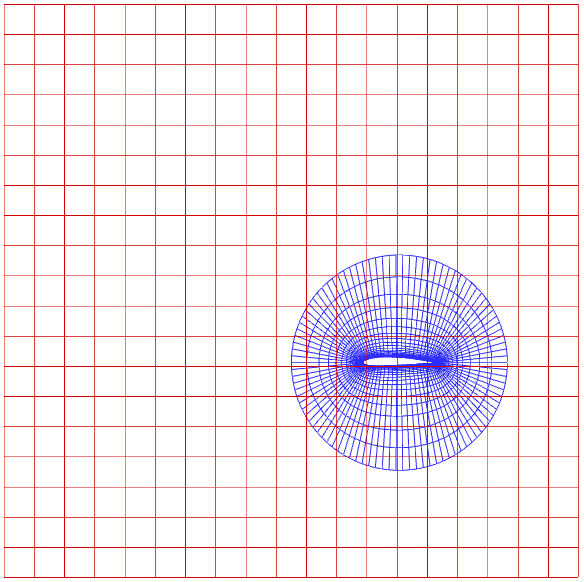
\includegraphics[width=0.3\linewidth]{figures/grid/chimera_grid}
  \caption{Chimera, overlapping grid for moving airfoil simulation}
  \label{f:chimera_grid}
\end{figure}


\subsubsection{Motivation for efficient wall distance computation}
Traditionally, the wall distance calculation would be of little
importance from an efficiency perspective. In stationary grid
simulations, the wall distance does not change, and so it would only
be performed once as a pre-processing step, which would represent a
trivial amount of time compared to the overall calculation. For moving
body simulations however, the wall distance can change after each
update of the body position and thus has to be recomputed for every
iteration. It becomes extremely important then, to have an efficient
method for recomputing the wall distance in order to maintain
reasonable computation times. Using graphics processing units(GPU's)
to accelerate the wall distance computation is seen as a promising
method for improving computational efficiency for moving body
problems.

\section{Design and optimization approach}
The application is laid out as a main function that consists of a
grid preprocessor, and then function calls to the respective wall
distance calculation routines. The preprocessor reads the
computational grid and stores the cell centers as two arrays,
$x$-coordinates and $y$-coordinates. It also reads in geometry faces and
stores their respective $x$ and $y$ coordinates in two separate
arrays. These are the input data to the wall distance calculation
routines. There are two wall distance calculation methods that are
being used for this investigation. They are a 'Brute Force' method and
'Advancing Boundary' method and will be described in the subsequent
sections. A diagram of the main application can be seen in Figure~\ref{f:main_application}.

\begin{figure}
  \centering
  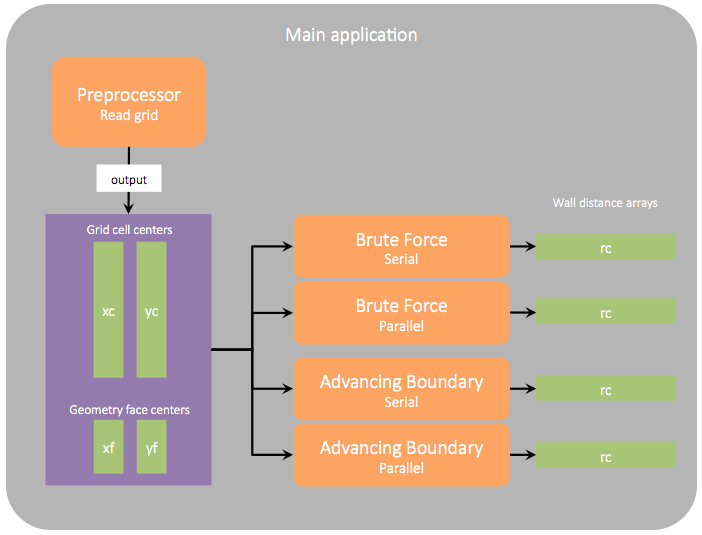
\includegraphics[width=0.6\linewidth]{figures/main_application_2}
  \caption{Main application diagram}
  \label{f:main_application}
\end{figure}


\subsection{Brute force method}

The brute force method for calculating the wall distance for a cell
element is shown in Figure~\ref{f:bf_1}.  For each cell element, its
distance from each of the solid faces is calculated (2D distance is
shown and used for this project).  Wall distance for the cell is the
minimum of these distances.

\begin{figure}
  \centering
  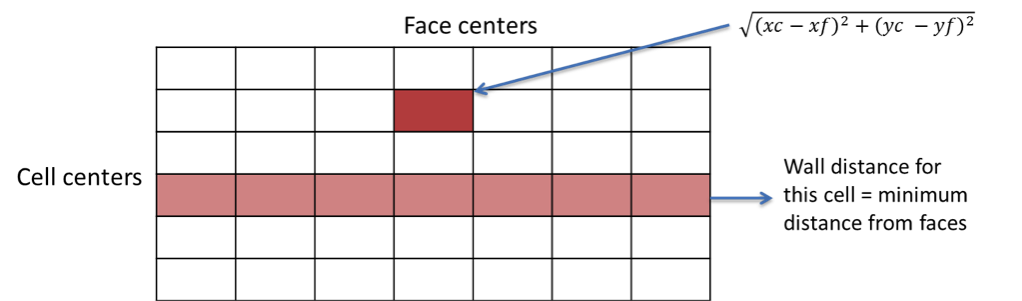
\includegraphics[width=0.7\linewidth]{figures/brute_force/bf_1}
  \caption{Brute force method}
  \label{f:bf_1}
\end{figure}


The serial implementation for the brute force method is shown in
Figure~\ref{f:bf_2}. For each cell element, the distance from the cell
to a large number of faces is calculated, and the wall distance is
updated if this face has the least distance. 

\begin{figure}
  \centering
  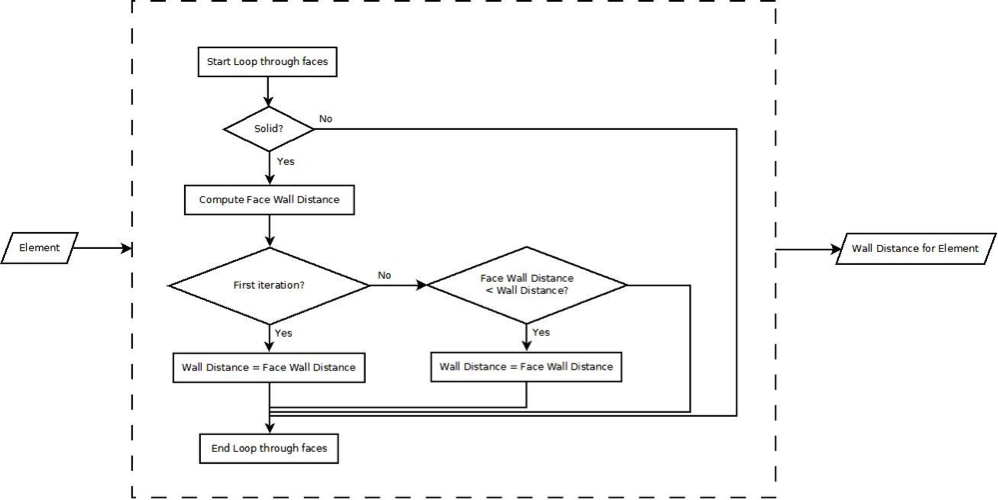
\includegraphics[]{figures/brute_force/bf_2}
  \caption{Brute force serial implementation}
  \label{f:bf_2}
\end{figure}



\subsubsection{Complexity}

The work and step complexities for the serial approach with $n$ cell
elements and $m$ solid faces can be approximated as: 

Work: O(n x m) – for each cell element, each solid face will have to
be evaluated.  So, total number of operations is in the order of n x
m. Step: O(m) – the cell elements can be evaluated in parallel, but the
distance from each solid face to the element is evaluated in sequence.
So, the longest chain of sequential dependencies is in the order of m.


\begin{itemize}
  
\item Work: O($n \times m$) - for each cell element, each solid face
  will have to be evaluated.  So, total number of operations is in the
  order of $n \times m$
  
\item Step: O($m$) - the cell elements can be evaluated in parallel,
  but the distance from each solid face to the element is evaluated in
  sequence.  So, the longest chain of sequential dependencies is in
  the order of $m$.
  
\end{itemize}

\subsubsection{Parallelization}
The opportunity for parallelism arises in being able to perform the
distance calculations and comparisons for each element and/or for each
face separately.  Two parallel approaches were implemented for the
brute force method.

\begin{enumerate}
  
  \item Block-per-cell (Figure~\ref{f:bf_3}): Each block (CUDA
    block) calculates the wall distance for a cell.  Each thread
    within a block calculates distance from a face; after all the
    threads have calculated the distance, a reduce minimum operation
    is performed to get the cell wall distance. 

  \item Thread-per-cell (Figure~\ref{f:bf_4}): Each thread calculates wall
    distance for a cell.  Each thread calculates distance from the
    cell to each of the faces, and keeps a “running” minimum distance
    value as each faces’ distance gets calculated. 

\end{enumerate}


\begin{figure}
  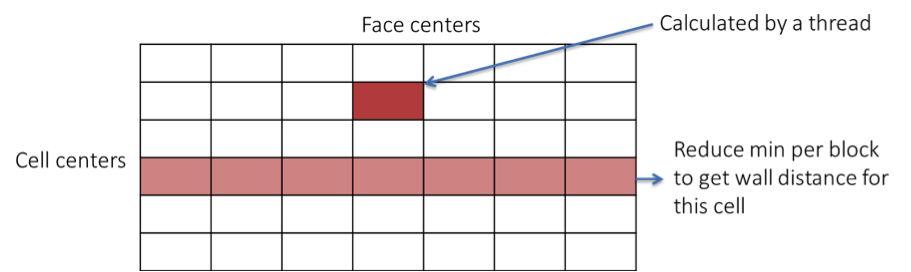
\includegraphics[]{figures/brute_force/bf_3}
  \caption{Brute force Block-per-cell implementation}
  \label{f:bf_3}
\end{figure}

\begin{figure}
  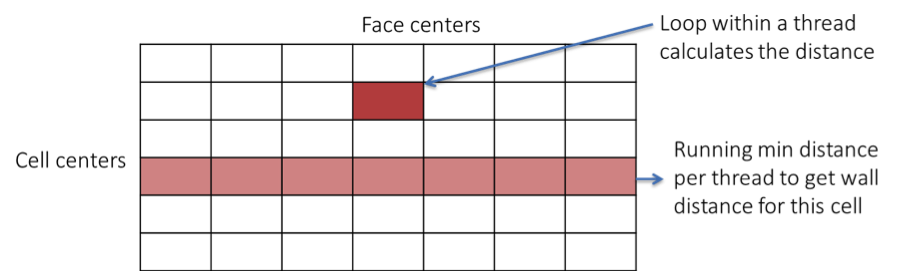
\includegraphics[]{figures/brute_force/bf_4}
  \caption{Brute force Thread-per-cell implementation}
  \label{f:bf_4}
\end{figure}


The work and step complexities for the parallel approaches with n cell
elements and m solid faces can be approximated as:

\begin{itemize}

\item Work: O($n \times m$) – work complexity for the two parallel
  implementations is similar to the serial implementation, as for each
  cell element, distance from each solid face will have to be
  evaluated.  So, total number of operations is in the order of $n
  \times m$.

\item Step: O($log_2 m$) for Block-per-cell, and O($m$) for
  Thread-per-cell – In the Block-per-cell implementation, the wall
  distances for each face can be calculated in parallel in one step,
  and the reduce operation to compute the minimum wall distance has a
  step complexity of $log_2 m$.  Therefore, step complexity for this
  parallel implementation is in order of $log_2 m$.  In the
  Thread-per-cell implementation, each of the cell elements can be
  evaluated in parallel in a separate thread, but the distance from
  each solid face to the element is evaluated in sequence inside each
  thread.  So, the longest chain of sequential dependencies is in the
  order of $m$.

\end{itemize}



\subsection{Advancing boundary method}
The ``Advancing Boundary'' method used in this investigation is based
on work done by Roget and Sitaraman, where they used
voxelized marching spheres to reduce the wall distance calculation to a small
subset of the original calculation.\cite{roget:12} The following process is largely the
same as the description in the paper, with modifications to auxiliary
cell structures and elimination of some of the more nuanced features.

The advancing boundary method begins with a preprocessing routine that
computes a set of auxiliary cells, which are then provided to the wall
distance calculation routine. This is shown
as a diagram in Figure~\ref{f:ab_preprocessor}.

\begin{figure}
  \centering
  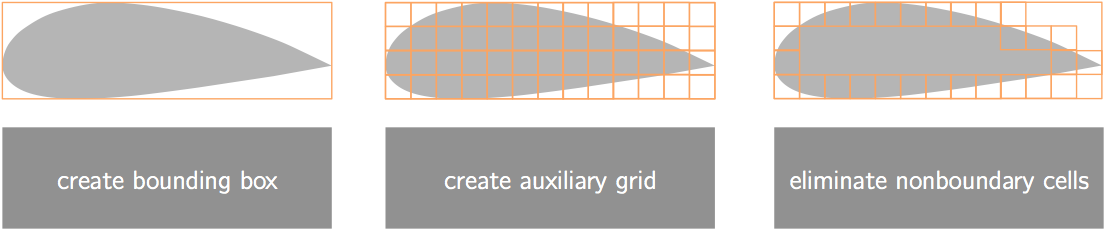
\includegraphics[width=0.6\linewidth]{figures/preprocessor/preprocessor_diagram}
  \caption{Advancing Boundary - Preprocessor}
  \label{f:ab_preprocessor}
\end{figure}


The goal of the auxiliary cells is that each would contain several
solid geometry faces. In this way, the wall distance routine can first
search through the smaller number of auxiliary cells to determine
those eligible for containing the closest solid face. This allows the
algorithm to reduce the number of total faces that need checked by
eliminating multiple solid faces each time an auxiliary cell is
eliminated. This wall distance calculation process is laid out in the diagram
in Figure~\ref{f:ab_diagram}.


\begin{figure}
  \centering
  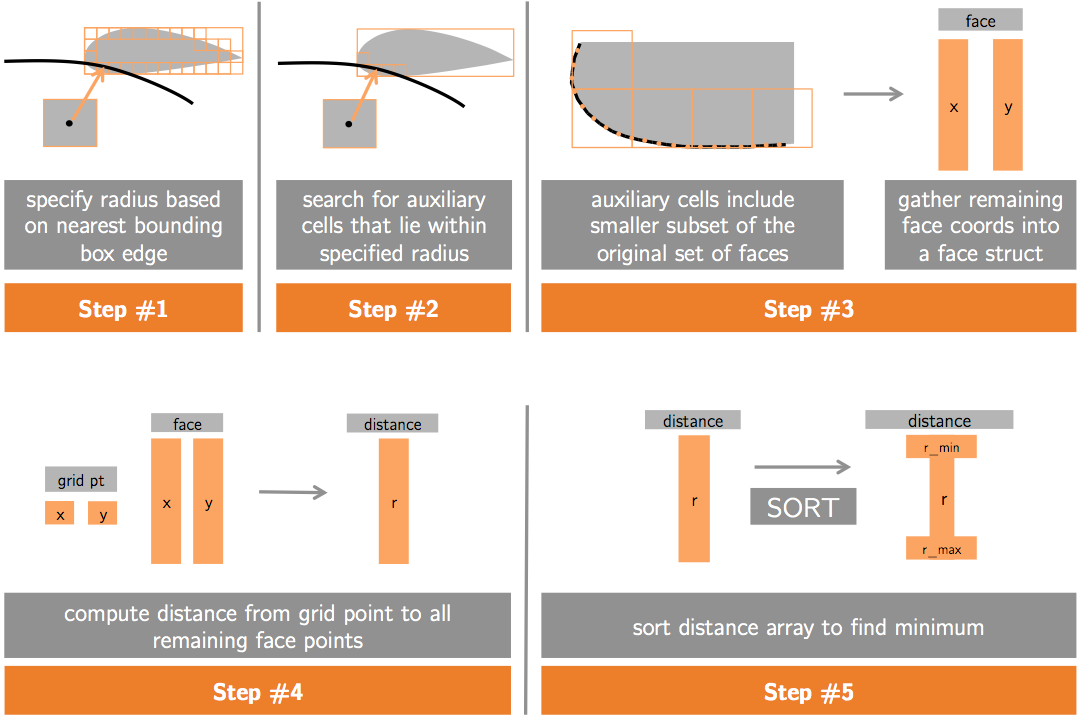
\includegraphics[width=0.7\linewidth]{figures/auxiliary_grid/algorithm_diagram}
  \caption{Advancing Boundary - Wall distance calculation}
  \label{f:ab_diagram}
\end{figure}



\subsubsection{Complexity}

The work complexity for this algorithm is related to the number of
cells in the computational grid and the number of solid geometry faces
that each cell has to search. In the worst case, each computational
grid must search through each solid face to find the closest
face. Therefore, for a case with $n$ computational cells and $m$ solid
geometry faces, the work complexity of the algorithm is O($n \times
m$). However, the computation for each cell executes independent of
all the other cells and requires, at worst, as many steps as there are faces, which is to search
through all of the solid geometry faces. As a result, the step
complexity of the algorithm is O($m$).

\subsubsection{Parallelization}
This algorithm, much in the same way as the brute force method, has a
lot of parallelism that can be exploited for improved
performance. Specifically, the wall distance calculation for each
computational cell executes independently of all other computational
cells. The parallel approach used for this study is a thread-per-cell
technique, where one wall distance kernel thread is launched for each
computational cell.


\begin{itemize}
\item Work: O($n \times m$)
\item Step: O($m$)
\end{itemize}


\section{Application performance and results}
The following sections present the methods used to benchmark each
algorithm, along with the various modifications implemented to improve
performance. Finally, timings for both serial and parallel
implementations are presented for both methods to evaluate the overall
speedup achieved via the parallel GPU implementation.


\subsubsection{Problem set}
The problem set chosen for this investigation was a solid circular
body, surrounded by a circular discretized domain. This simple
geometry allowed a computational grid to be easily refined in order to
load algorithms more heavily and reduce the effect of computational
overhead on the overall timings. The grid and wall distance field can
be seen in Figure~\ref{f:circle}.

\begin{figure}
  \centering
  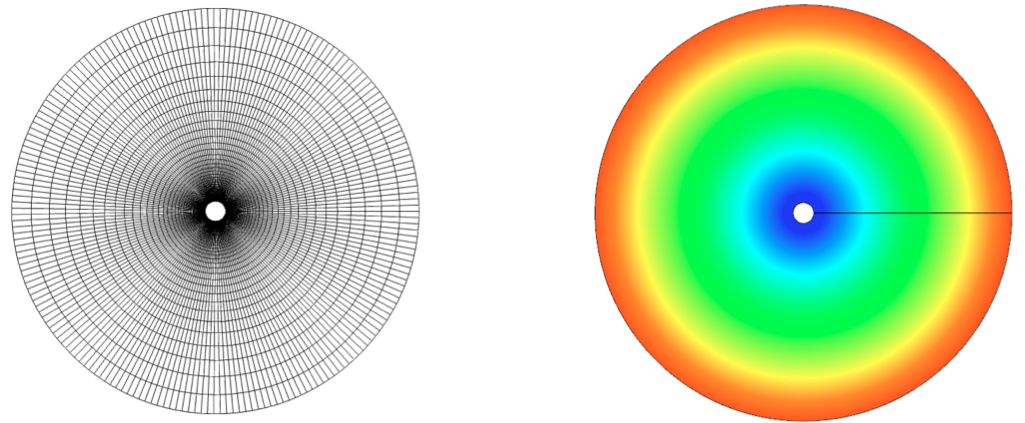
\includegraphics[width=0.7\linewidth]{figures/grid/circle_grid}
  \caption{Computational grid and corresponding wall distance field}
  \label{f:circle}
\end{figure}


\subsubsection{Brute-force algorithm}

Several implementations of the two brute force parallel methods were
tested in order to evaluate efficient memory usage such as coalesced
memory access, use of available shared memory and thread local
memory. 

Three variations of the Block-per-cell method were implemented:

\begin{enumerate}

  \item 1A: Shared memory writes for face distances – since a
    reduce operation per block is performed to get the minimum
    distance from an array of distances calculated by the threads, the
    distance array is stored in shared memory.

  \item 1B: (1A) + Shared memory reads to face ($x, y$) arrays – storing
    the face ($x, y$) arrays in shared memory, so that every thread does
    not have to read all of the face ($x, y$) arrays from global memory.

  \item 1C: Same as (1B) with ($x, y$) arrays converted to an
    interspersed array for coalesced shared memory reads, i.e. $x0, y0,
    x1, y1, ....$

\end{enumerate}


Three variations of the Thread-per-cell method were implemented:

\begin{enumerate}
  
\item 2A: Each thread calculates wall distance for a cell.
  
\item 2B: Shared memory reads to face ($x, y$) arrays.
  
\item 2C: Same as (2A) with ($x, y$) arrays converted to an
  interspersed array for coalesced global memory reads, i.e. $x0, y0,
  x1, y1, ....$
  
\end{enumerate}


The performance of the different brute force parallel methods is shown
in Table~\ref{t:bf_performance}.  The times shown are based on several sample runs of the
algorithm on the Ohio Supercomputer Center (OSC) Oakley cluster. 


\begin{table}% no placement specified: defaults to here, top, bottom,
             % page
  \centering
 \begin{center}
  \caption{Brute force algorithm performance}
  \label{t:bf_performance}
%  \begin{tabular}{ccccc}
  \begin{tabular}{m{5cm} c c c c}
    \multicolumn{1}{m{5cm}}{\centering Algorithm} & SM Grid($ms$) & MD Grid($ms$) & FN
                                                           Grid($ms$) &
                                                                      Speedup(FN
                                                                      vs Ser.)\\\hline\hline

    \multicolumn{1}{m{5cm}}{\centering Serial} & 33 & 595 & 13636 & Not applicable \\\hline
    \multicolumn{1}{m{5cm}}{\centering Block-per-cell(1A):\\Shared
    memory writes} & 1 & 28 & - & - \\\hline
    \multicolumn{1}{m{5cm}}{\centering Block-per-cell(1B):\\Shared
    memory reads} & 1 & 30 & - & - \\\hline
    \multicolumn{1}{m{5cm}}{\centering Block-per-cell(1C):\\Coalesced
    shared memory reads} & 1 & 31 & - & - \\\hline
    \multicolumn{1}{m{5cm}}{\centering Thread-per-cell(2A)\\} & $<1$ &
                                                                    7&173 & 79 \\\hline
    \multicolumn{1}{m{5cm}}{\centering Thread-per-cell(2B):\\Shared
    memory reads} & 1 & 9 & 293 & 46 \\\hline
    \multicolumn{1}{m{5cm}}{\centering Thread-per-cell(2C):\\Coalesced
    global memory reads} & $<1$ & 7 & 166 & 82 \\\hline
\hline
  \end{tabular}
 \end{center}
\end{table}



The Block-per-cell methods do not support grid sizes with a large
number of faces, as these methods require the number of faces to be
less than the maximum number of threads available per block (1024 for
the OSC cluster).  Therefore, performance could not be measured for
the extra fine grid.  Also, the overhead of setting up shared memory
and coalesced reads outweighs the performance gains for the small/fine
grid sizes (1B and 1C).  Therefore, performance for all three
Block-per-cell methods was similar for the small/fine grid sizes.


The Thread-per-cell methods performed better than the Block-per-cell
methods.  Also, the Thread-per-cell methods do not have limitations on
the grid size, and can accommodate any grid size.  Thread-per-cell is
not a good algorithm for utilizing shared memory, since each thread
has to calculate the wall distance for a cell.  However, this method
(2B) was implemented in order to access if there is a performance gain
from one thread in a block reading the face values and storing them in
shared memory, instead of all threads reading them from shared memory.
As expected, this caused a negative impact on performance due to
thread divergence, as one thread had to perform significantly large
amount of work compared to all the other threads in the block.  The
coalesced global memory reads made a slight improvement in
performance, since reading the blocks in a coalesced manner reduces
the memory access time.  Therefore, the Thread-per-cell method with
coalesced global memory reads (2C) was the optimal brute force
algorithm implemented in this project, with a speed-up of 82 compared
to the serial method.


For future improvements, a combination of the Thread-per-cell and
Block-per-cell methods can be used in order to achieve the best
possible performance (as close to O($log_2 m$) as possible).  This can be
done by separating out the two main calculations into two steps:
calculating the face distances from the cell centers in one kernel,
with each thread calculating a distance (i.e. “thread-per-cell face
distance”); and then assigning blocks so that each block performs a
reduce minimum on the face distances related to a cell
(i.e. “block-per-cell reduce).  This will require a block/thread
sizing algorithm that can handle the different grid sizes.  Another
future improvement that should be explored is to break up the grid
calculations into tiles, as that helps with efficient memory reads. 


















\subsubsection{Advancing boundary algorithm}
Several implementations of the advancing boundary algorithm were
tested, both for serial and parallel algorithms. The different methods
for improving performance included memory management and changing storage
structures. The initial serial algorithm was implemented with an
'Auxiliary Cell' struct that would include the geometric information
for a given auxiliary cell, in addition to providing some method for
accessing the faces that were contained in the face. The general
layout of this struct was similar for all iterations of the serial and
parallel codes. Only the face storage mechanism was altered for more
efficient memory accesses. The first iteration of these stored the
faces as a linked-list of face structs, each of which stored the x,y
pair associated with a face center. This initial configuration is shown in
Figure~\ref{f:initial_aux_cell}.

\begin{figure}
  \centering
  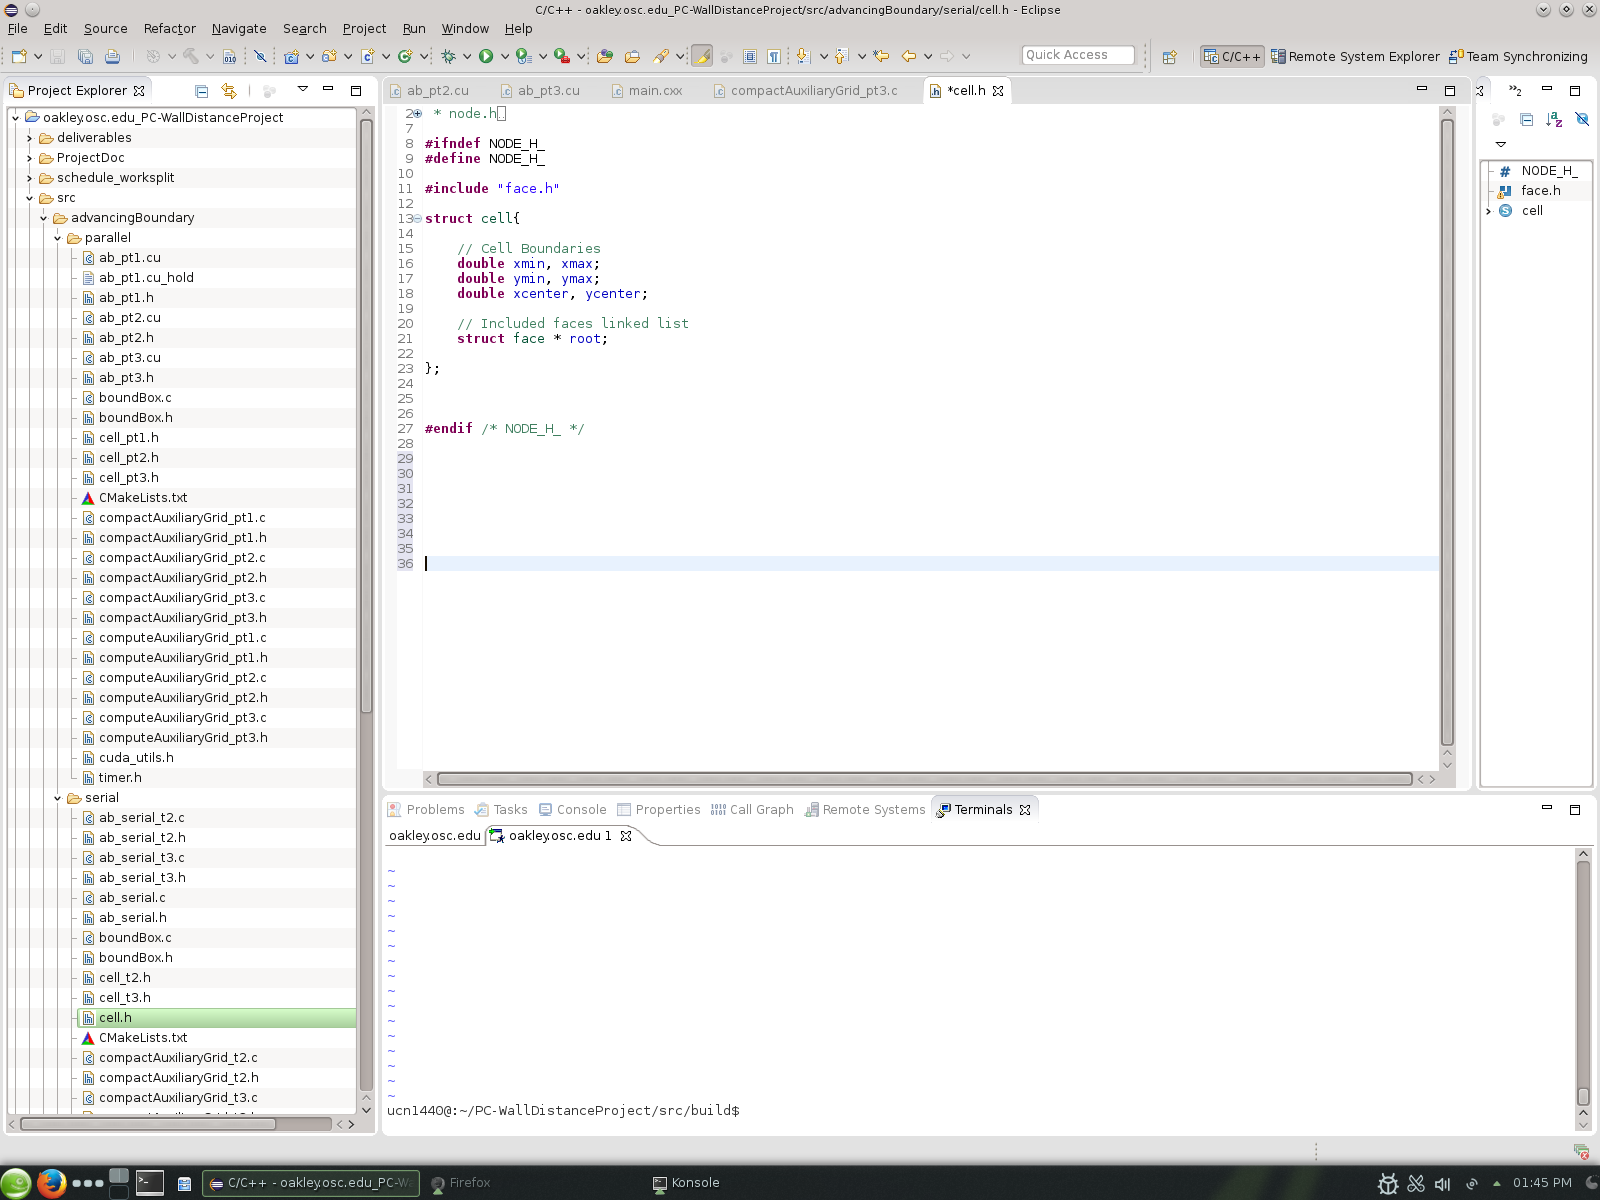
\includegraphics[trim=11.2cm 21.8cm 24cm 5.2cm,
  clip=true, width=0.3\linewidth]{figures/cells/cell_linked_list}
  \caption{Initial auxiliary cell struct}
  \label{f:initial_aux_cell}
\end{figure}

Other methods for storing the faces included pointers to face arrays,
explicitly allocated arrays in the cell struct, and also an array of
face indices that would facilitate access to the correct face in an
external array.

\begin{figure}
  \begin{subfigure}[b]{0.45\linewidth}
    \centering
    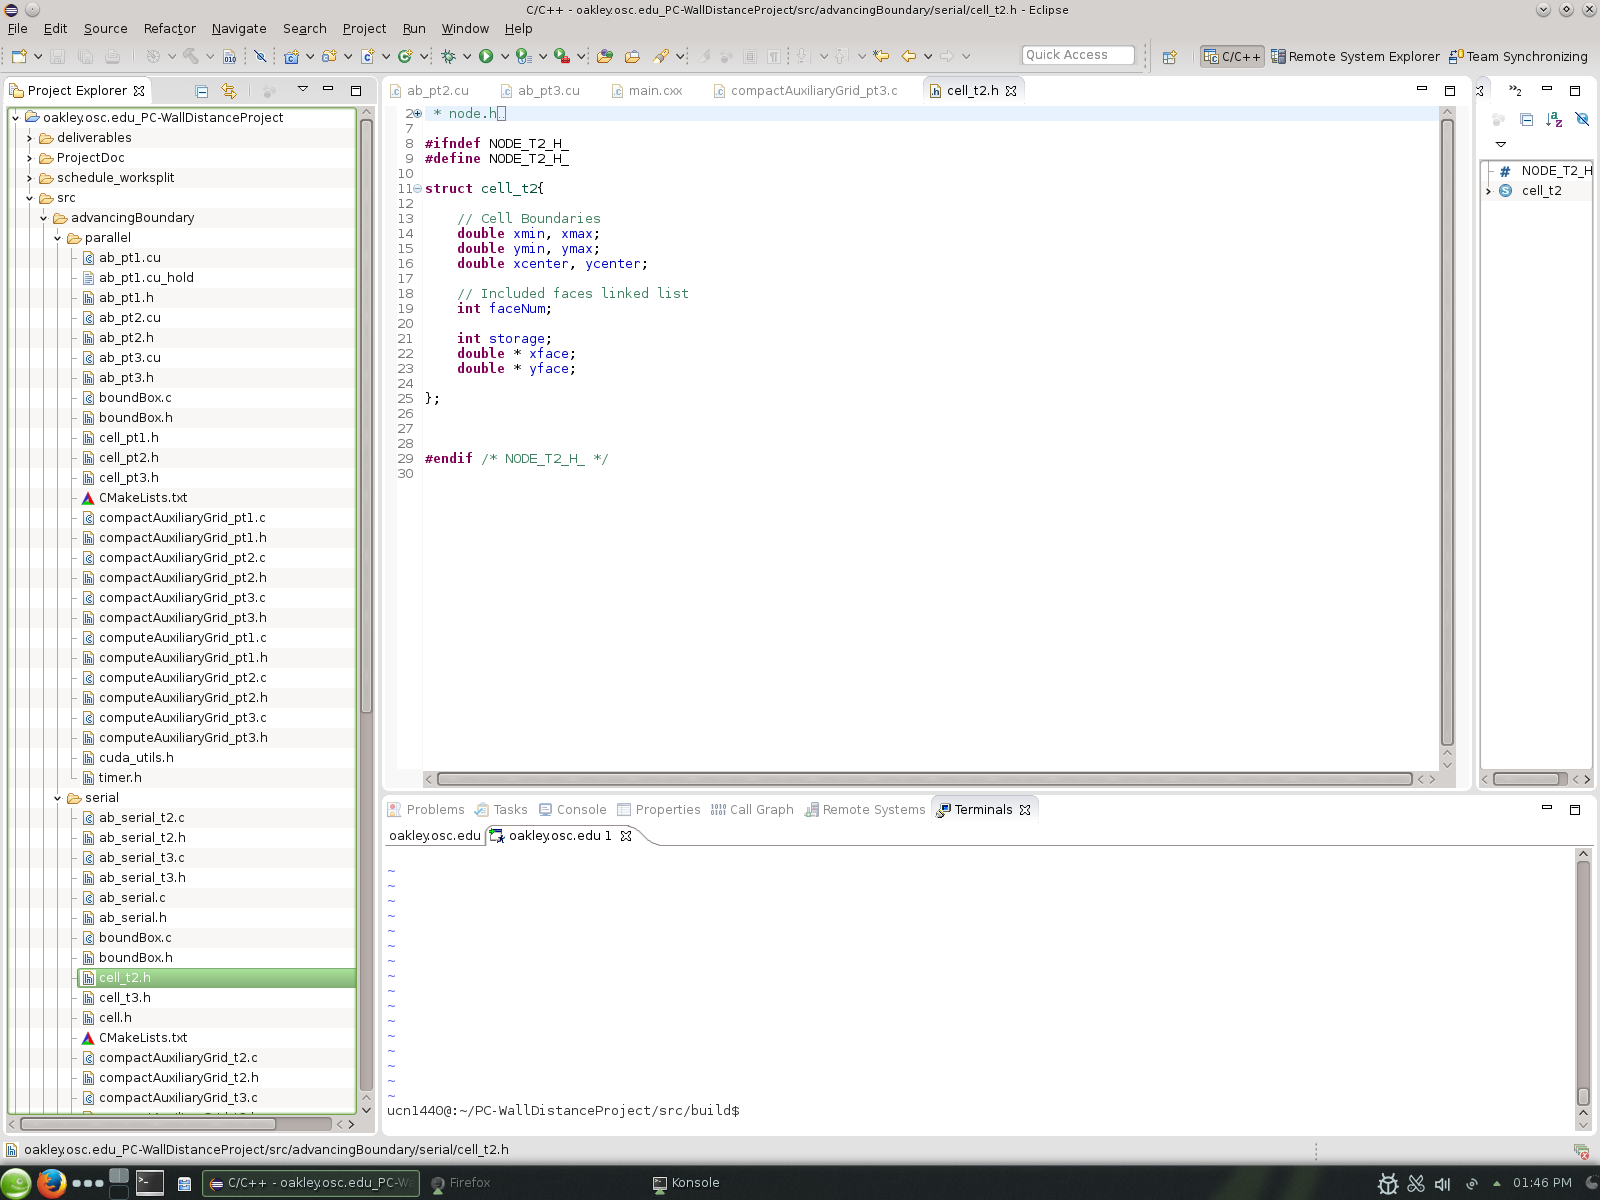
\includegraphics[trim=11.2cm 21.8cm 24cm 4.8cm,
    clip=true, width=0.7\linewidth]{figures/cells/cell_pointers}
    \caption{Struct A: Pointers to storage arrays}
  \end{subfigure}
  ~
  \begin{subfigure}[b]{0.45\linewidth}
    \centering
    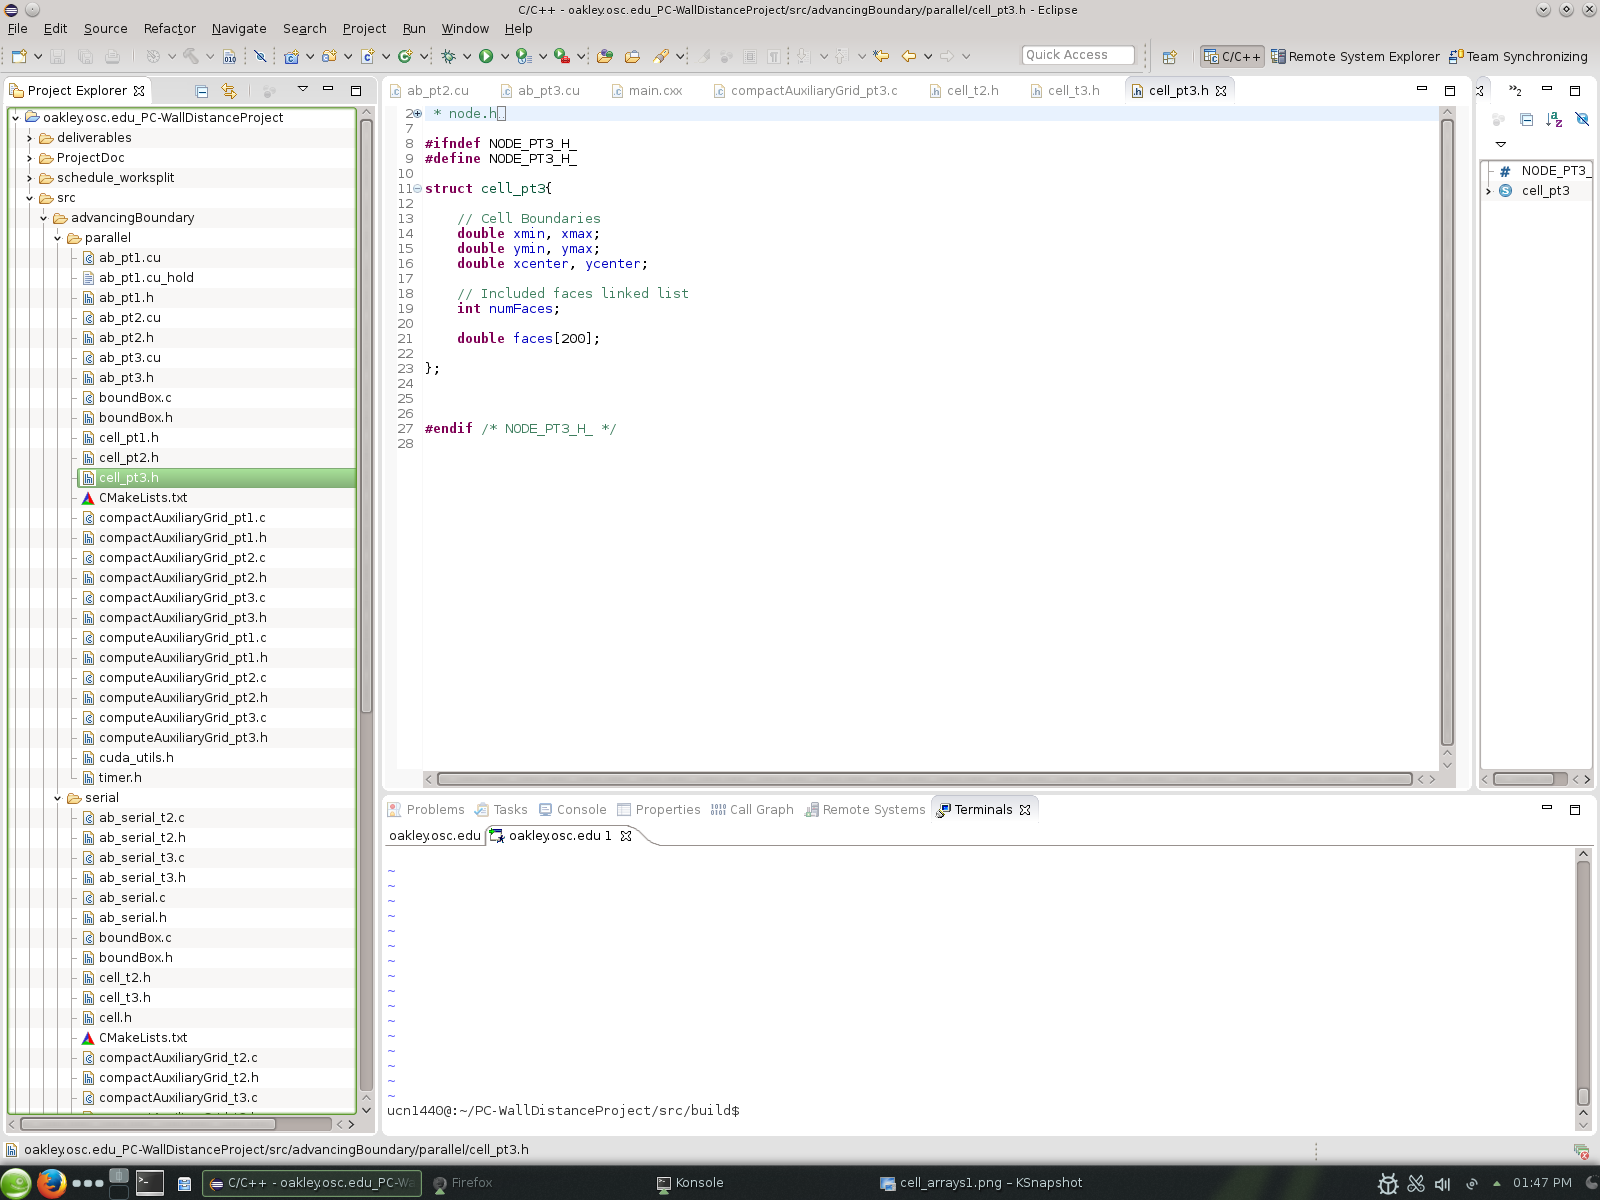
\includegraphics[trim=11.2cm 21.8cm 24cm 4.8cm,
    clip=true, width=0.7\linewidth]{figures/cells/cell_array}
    \caption{Struct B: Explicitly allocated in-cell storage}
  \end{subfigure}
  
  \begin{subfigure}[b]{0.45\linewidth}
    \centering
    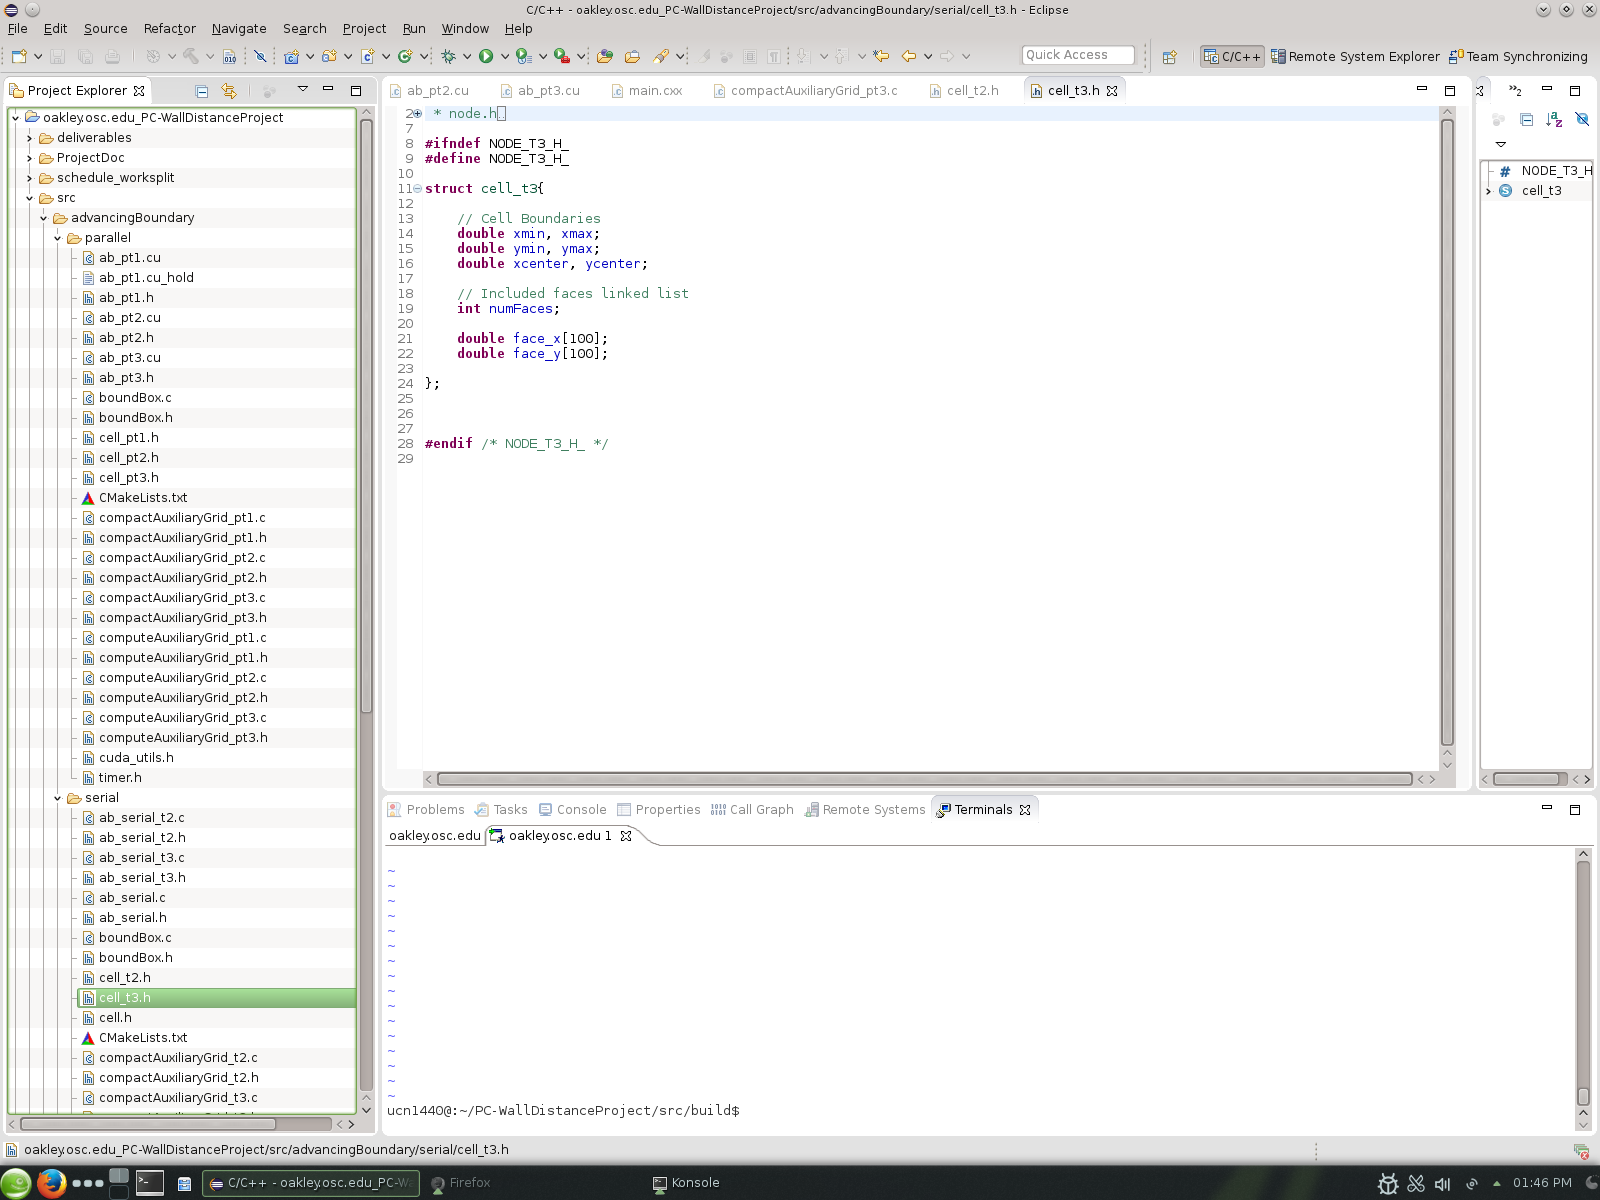
\includegraphics[trim=11.2cm 21.8cm 24cm 4.8cm,
    clip=true, width=0.7\linewidth]{figures/cells/cell_arrays}
    \caption{Struct C: Separate in-cell storage}
  \end{subfigure}
  ~
  \begin{subfigure}[b]{0.45\linewidth}
    \centering
    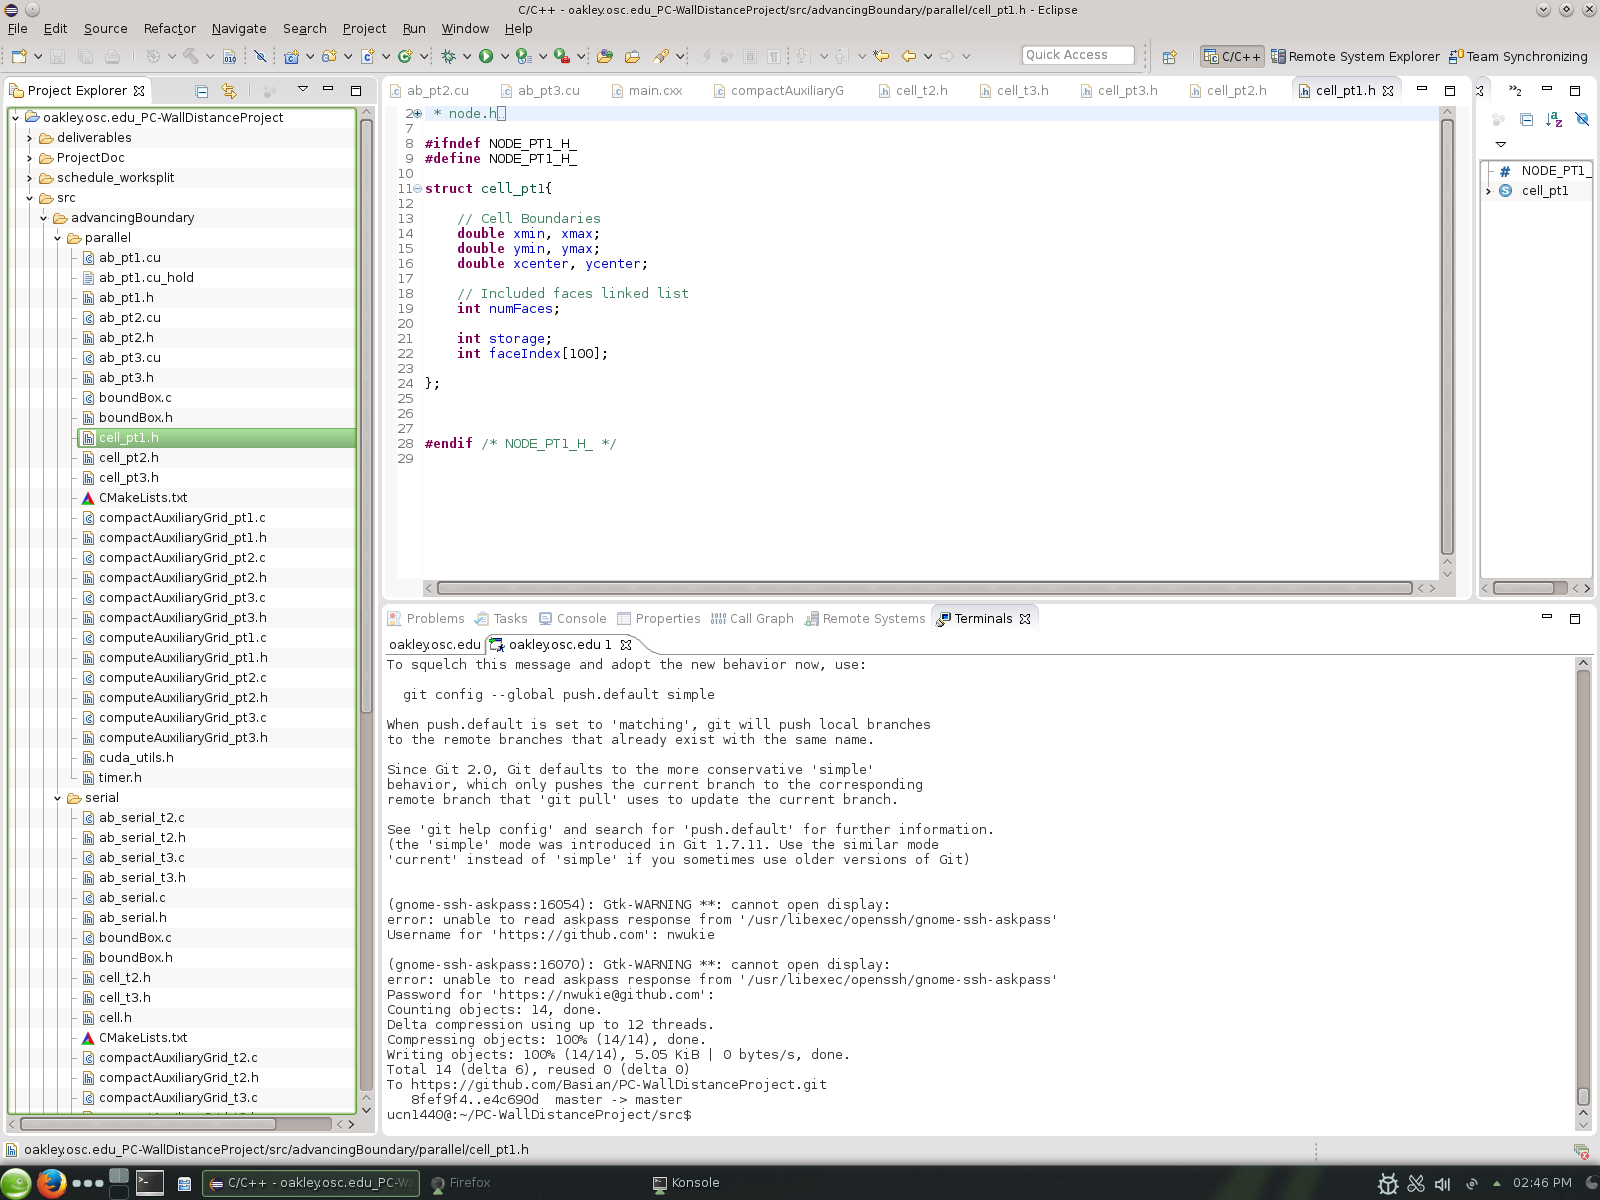
\includegraphics[trim=11.2cm 21.8cm 24cm 4.8cm,
    clip=true, width=0.7\linewidth]{figures/cells/cell_index}
    \caption{Struct D: Face index array}
  \end{subfigure}
  
  \caption{Auxiliary cell struct versions}
\end{figure}


The timings for the Serial algorithm are shown in
Table~\ref{t:serial}. The linked-list method of storing faces was the
most efficient access method of those tested. The best-performing
serial algorithm was then compared to the parallel algorithms to gauge
the parallel speedup factor. The parallel timings are shown in
Table~\ref{t:parallel}. The initial implementation used all global
memory accesses and subsequent improvements focused on bringing in
reusable data into shared memory or local registers. Some final
performance improvements were achieved by restructuring the face
storage structure.

\begin{table}[h]
  \centering
  \begin{tabular}{ccc}
    Iteration & Description & Average Time (ms) \\
    \hline\hline
    T1 & Baseline, linked-list of faces & 8796 \\
    T2 & New aux cell struct & 11044 \\
    T3 & New aux cell struct & 10007 \\
    \hline
  \end{tabular}
  \caption{Serial ``Advancing Boundary'' algorithm development and performance}
  \label{t:serial}
\end{table}



\begin{table}[h]
  \centering
  \begin{tabular}{cccc}
    Iteration & Description & Average Time (ms) & Speedup vs. Serial\\
    \hline\hline
    T1 & Baseline, no shared memory & 134 & 65\\
    T2 & Memory management & 114 & 77\\
    T3 & Memory management & 114 & 77\\
    T4 & Memory management & 112 & 78\\
    T5 & Memory management & 113 & 78\\
    T4 - new cell - 1 & New aux cell struct & 106 & 83\\
    T4 - new cell - 2& New aux cell struct & 102 & 86\\
    \hline
  \end{tabular}
  \caption{Parallel ``Advancing Boundary'' algorithm development and performance}
  \label{t:parallel}
\end{table}



\section{Schedule and division of work}
Figure~\ref{f:schedule} shows the work split between the team contributors.

\begin{figure}
  \centering
  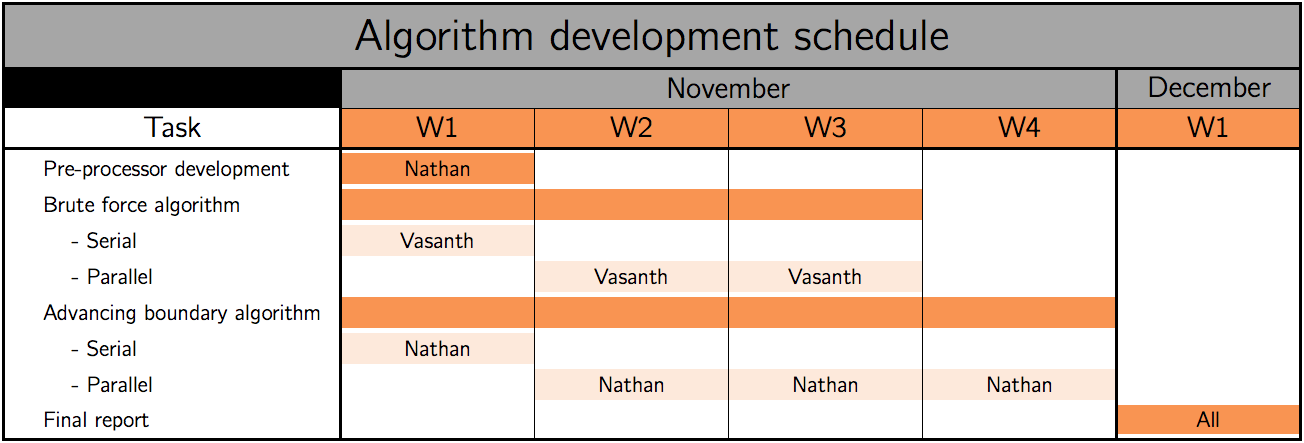
\includegraphics[width=0.9\linewidth]{figures/schedule_update}
  \caption{Development schedule and division of work}
  \label{f:schedule}
\end{figure}


\subsection{Self-assessment: Nathan Wukie}
I provided the primary topic and guidance for the project, along with
the application framework, preprocessor, and cmake
usage. Additionally, I was responsible for the ``Advancing Boundary''
algorithm development, implementation, and parallelization.

\subsection{Self-assessment: Vasanth Ganapathy}
I was responsible for the “Brute Force” algorithm development,
implementation, and testing.  This includes the serial and parallel
methods for the “Brute Force” algorithm.  





% produces the bibliography section when processed by BibTeX
\nocite{*}
\bibliography{bibliography}
\bibliographystyle{aiaa}


\clearpage
\begin{appendices}
  \section{Source code}
  \noindent
  The source code and all supporting documents used for this project
  can be accessed through the following git repository:
  \\\\
  \noindent
  https://github.com/Basian/PC-WallDistanceProject.git

  \section{Presentation slides}
  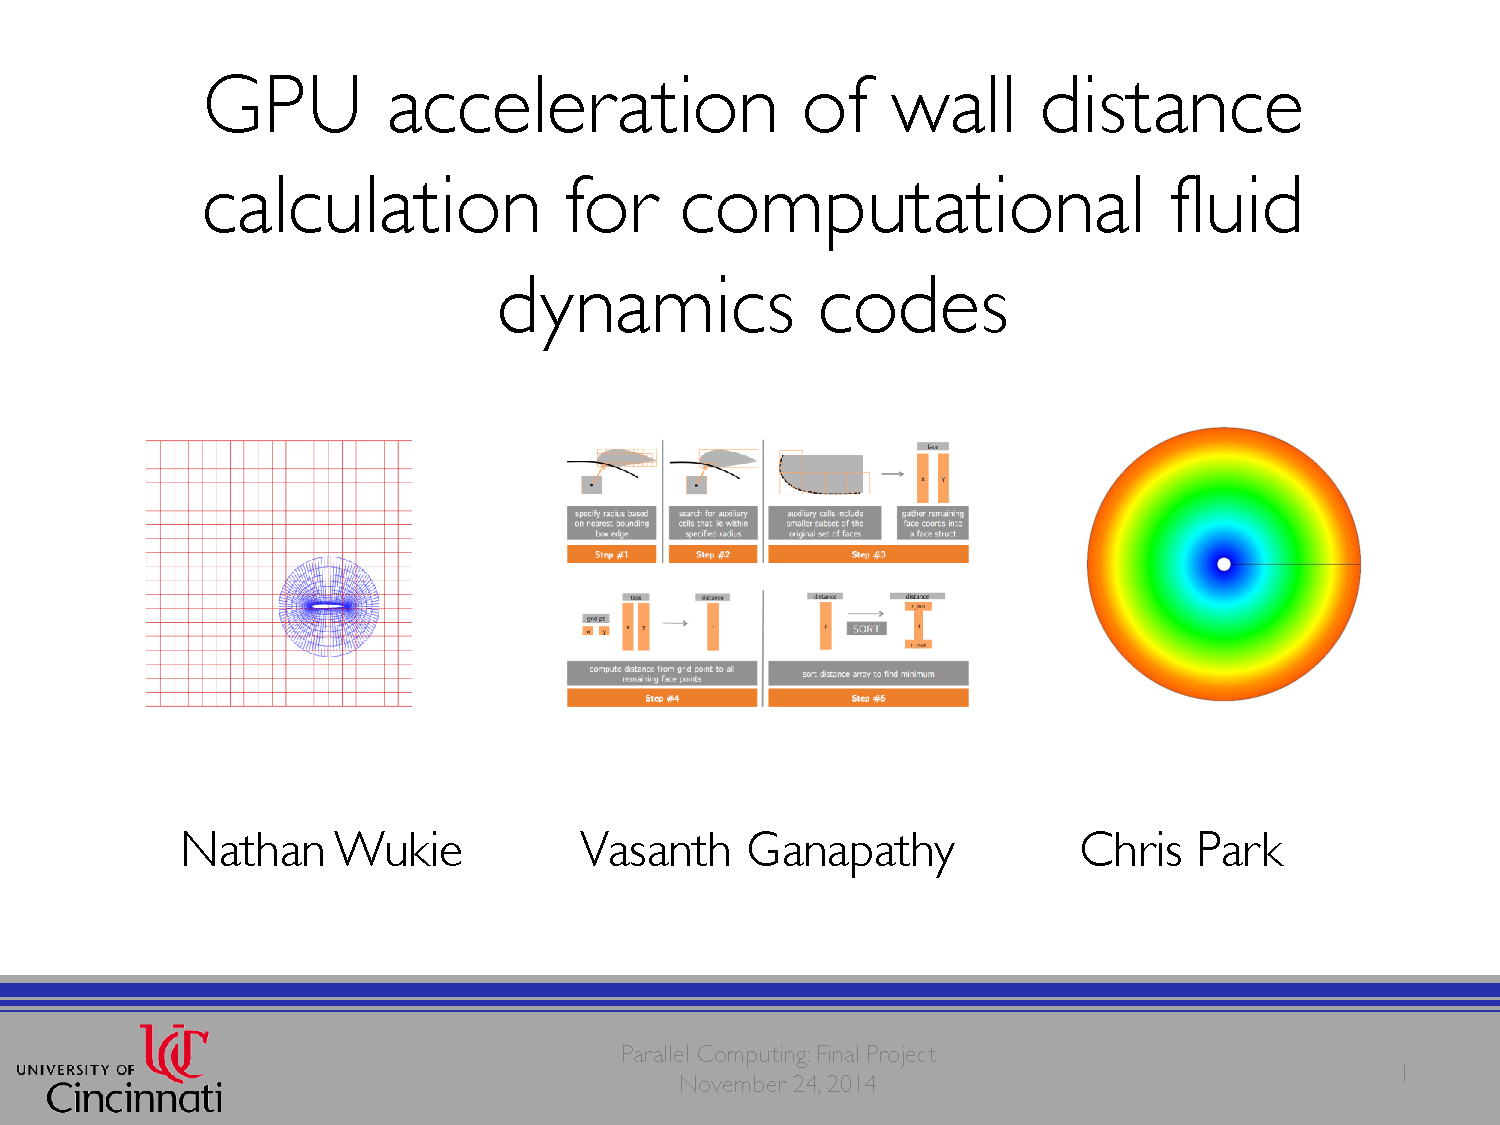
\includepdf[nup=1x2,pages=-]{slides/assembled_final}

\end{appendices}

\end{document}

% - Release $Name:  $ -
